\documentclass{article}

% if you need to pass options to natbib, use, e.g.:
%     \PassOptionsToPackage{numbers, compress}{natbib}
% before loading neurips_2021

% ready for submission

% to compile a preprint version, e.g., for submission to arXiv, add add the
% [preprint] option:
%     \usepackage[preprint]{neurips_2021}

% to compile a camera-ready version, add the [final] option, e.g.:
\usepackage[final]{workshop}

% to avoid loading the natbib package, add option nonatbib:
%    \usepackage[nonatbib]{neurips_2021}

\usepackage{wrapfig}
\usepackage{graphicx}
\usepackage{fontawesome}

\usepackage[utf8]{inputenc} % allow utf-8 input
\usepackage[T1]{fontenc}    % use 8-bit T1 fonts
\usepackage{hyperref}       % hyperlinks
\usepackage{url}            % simple URL typesetting
\usepackage{booktabs}       % professional-quality tables
\usepackage{amsfonts}       % blackboard math symbols
\usepackage{nicefrac}       % compact symbols for 1/2, etc.
\usepackage{microtype}      % microtypography
\usepackage{xcolor}         % colors

\usepackage{float}
\usepackage{pgf}
\usepackage{tikz}
\usetikzlibrary{arrows,automata}

\title{Advances in Programming Languages\\ and Neurosymbolic Systems (AIPLANS)}

% The \author macro works with any number of authors. There are two commands
% used to separate the names and addresses of multiple authors: \And and \AND.
%
% Using \And between authors leaves it to LaTeX to determine where to break the
% lines. Using \AND forces a line break at that point. So, if LaTeX puts 3 of 4
% authors names on the first line, and the last on the second line, try using
% \AND instead of \And before the third author name.

\author{%
    Breandan Considine$^{1, 4}$, Disha Shrivastava$^{1, 3, 4}$, David Yu-Tung Hui$^{2, 4}$ \\
    \textbf{Chin-Wei Huang$^{2, 4}$, Shawn Tan$^{2, 4}$, Xujie Si$^{1, 4}$, Prakash Panangaden$^{1, 4}$} \\
    McGill University$^1$, Universit\'e de Montr\'eal$^2$, Google$^3$, Mila$^4$ \\
    \texttt{\{considib, shrivast, huidavid, huangchi, tanjings,}\\
    \texttt{xujie.si, prakash.panangaden\}@mila.quebec} \\
}

\begin{document}

    \maketitle

    \begin{abstract}
        Automatic differentiation libraries and frameworks have enabled much progress in gradient-based learning over the last decade. Recent domain-specific languages for automatic programming hold the promise of unleashing similar progress in e.g., probabilistic and classical reasoning. Concurrently, machines have made steady progress in representing and synthesizing programs. Other workshops have explored these themes separately, yet few have highlighted the synergies between automatic and synthetic programming, a situation we hope to remedy.
    \end{abstract}


    \section{Proposal}

    Neural information processing systems have benefited tremendously from the availability of programming languages and frameworks for automatic differentiation. Similar domain-specific languages have shown progress automating inference in other logical disciplines, such as belief nets, proof nets, and related message passing schemes on tree- and graph-structured data.

    Not only does machine learning itself benefit from languages for programmable inference, these systems can also be seen as a kind of low-level programming language in their own right, consisting of differentiable and stochastic primitives. While currently less interpretable, thanks to recent progress in statistical language modeling, these systems are increasingly capable of generating symbolic functions resembling procedures a human programmer might plausibly write in a high-level language.

    Applying techniques from programmable inference to transform and generate programs, and adapting insights gained developing those same programs to drive innovation in higher-order AD and probabilistic programming is a virtuous cycle, with a growing stream of software and academic papers. We envision cooperation between automatic and synthetic programming will continue to increase as researchers become more accustomed to outsourcing low-level reasoning tasks to these systems.

    \begin{figure}[H]
        \centering
        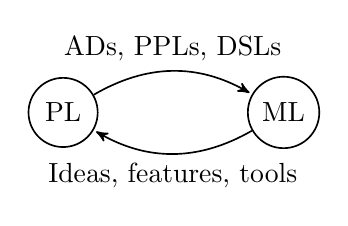
\begin{tikzpicture}[->,>=stealth',shorten >=1pt,auto,node distance=2.8cm, semithick]
%        \tikzstyle{every state}=[draw=none,text=white]

            \node[state]         (A)                    {PL};
            \node[state]         (B) [right of=A]       {ML};

            \path (A) edge [bend left] node {ADs, PPLs, DSLs} (B)
            (B) edge [bend left] node {Ideas, features, tools} (A);
        \end{tikzpicture}
    \end{figure}

    Many ideas are being reinvented and rediscovered in this process. AD itself was invented a half dozen times over the last century and research continues to reveal unexpected connections to implicit differentiation, bilevel optimization, optimal control, stochastic processes and differential equations. Semiring programming has existed in various forms for many decades and shares deep connections to reinforcement learning, structured inference and probabilistic programming. Much work remains.

    Likewise, many recently-transplanted ideas in machine learning are catechism in the programming language literature. For example, functional and type-safe programming are lingua franca in PL circles but relatively new to Python, the primary language used in machine learning. The duality between code and data is well-known in PL under the aegis of homoiconicity. PL theory has thought deeply about categorical semantics, concurrency, process calculi, linear logic, privacy and other deeply useful concepts which remain, to this day, mostly unfamiliar in the machine learning community.

%    Similarly, the programming language community too, has its blind spots. PLs have long wrestled with the distinction between intensional and extensional representation, a distinction which the statistical learning community has long since reconciled under the umbrella of model-based learning and approximation theory. PL could take a page from structured inference and propagation algorithms as a medium for distributed computation. We believe many other such examples await discovery.

    Other areas where the interaction could be fruitful are tools for equivalence, proof search and metrics. A deeper understanding of programming language semantics are largely missing from neural program synthesis discussions. The connection between various forms of message passing in concurrent systems and neural science merits further investigation. New language models could enable more effective tools for natural language and assistive programming. While some of these topics remain greenfield research topics, many connections are known, but yet-to-be-translated textbook knowledge.

    As outlined above, we believe that recent advances in statistical learning and programming languages have been largely siloed, but these two communities have many ideas yet to share. In exchange, we believe a great deal of progress can be achieved, in particular, between automatic and synthetic programming. A joint workshop such as the one put forward in this proposal could help to facilitate yet-unrealized research connections among neighboring fields. Our workshop is designed to be as inclusive as possible towards researchers of various backgrounds working on programming languages and neurosymbolic systems. For illustration, we include the following incomplete list of topics:

    \begin{itemize}
        \item Differentiable programming / algorithmic differentiation
        \item Probabilistic programming / statistical inference
        \item Dynamic programming / reinforcement learning
        \item Program induction / program synthesis
        \item Functional programming / $\lambda$-calculus
        \item Semiring programming / message passing
        \item Array programming / linear algebra
        \item Logic programming / Relational programming
        \item Meta-programming / meta-learning
        \item Computer aided reasoning / automatic theorem proving
        \item Domain-specific languages and compilers
        \item Inductive programming / programming by example
    \end{itemize}

    The workshop will be a single-day event hosted online, enabling an economically and geographically diverse audience to participate. Talks will be hosted in English, following the standard format of oral presentations and panel discussions, to be concluded with a virtual poster session. Outside of standard videoconferencing and SlidesLive assistance, we anticipate no other technical requirements. If accepted, we expect to receive an audience a hundred or so participants, including speakers and workshop submitters, based on attendance at similarly-themed workshops in prior years.

    We would like to encourage developers of languages, frameworks and libraries to submit their work for evaluation. Those who traditionally publish in venues such as SIGPLAN and SIGSOFT are also encouraged to submit work that may be relevant to the machine learning and reasoning community, provided that effort is taken to ensure its accessibility. Special consideration will be given to didactic submissions of outstanding clarity. Further information, including evaluation criteria, examples of relevant literature, deadlines and workshop logistics will be made available in a timely manner.

    AIPLANS celebrates cultural, linguistic, ethnic and intellectual diversity as demonstrated by its organizers' own unique backgrounds. Not only are we committed to nondiscrimination on the basis of, e.g., race, creed, age, gender, orientation, phyiscal or mental handicap, but also aim to encourage individuals from other disadvantaged and underrepresented socioeconomic backgrounds to participate. Should our workshop be accepted, scholarships covering the cost of registration will be provided for those who wish to attend but would otherwise be unable to do so due to financial hardship.

    \textbf{Tagline:} Are you curious whether machines can write programs that are both sound and interpretable? Come check out AIPLANS, a new workshop on domain-specific languages for learning and synthetic reasoning, to be hosted at NeurIPS 2021! \url{https://aiplans.github.io}

    \newpage


    \section{Organizers}

    \begin{figure}[H]
        \begin{wrapfigure}{l}{0.2\textwidth}
            \includegraphics[width=0.2\textwidth]{organizers/breandan}
        \end{wrapfigure}
        \textbf{Breandan Considine} is a Ph.D. student at McGill University. His research studies the relationship between software and machine learning, to reason about the behavior of real-world programs and use those insights to build more intelligent programming tools for developers. Previously, Breandan obtained his  Master's degree under the supervision of Liam Paull and Michalis Famelis, where he studied differentiable programming and software engineering. He is enthusiastic about AI as a tool for augmenting human reasoning.\\
        \faHome: \url{https://breandan.github.io/} \faTwitter: \href{https://twitter.com/breandan}{@breandan}
    \end{figure}

    \begin{figure}[H]
        \begin{wrapfigure}{l}{0.2\textwidth}
            \includegraphics[width=0.2\textwidth]{organizers/disha}
        \end{wrapfigure}\textbf{Disha Shrivastava} is a Ph.D. student in Machine Leaning at Mila, working with Hugo Larochelle and Danny Tarlow. She also works part-time at Google Brain, Montreal as a Student Researcher. Earlier, she worked at IBM Research, India as a Research Software Engineer for two years. Her work focuses on unsupervised construction of knowledge graphs, metrics for computational creativity and topical coherence and reasoning for maths question-answering. Previously, she graduated from IIT Delhi with a Masters in Computer Technology, where she developed a data and model-parallel framework for training of deep networks in Apache Spark. Disha's current areas of research includes program understanding and generation, meta-learning, compositional generalization and developement of reasoning-based systems for QA tasks.\\
        \faHome: \url{https://shrivastavadisha.github.io/} \faTwitter: \href{https://twitter.com/dishaShrivasta9}{@dishaShrivasta9}
    \end{figure}

    \begin{figure}[H]
        \begin{wrapfigure}{l}{0.2\textwidth}
            \includegraphics[width=0.2\textwidth]{organizers/david}
        \end{wrapfigure}\textbf{David Yu-Tung Hui} is a MSc student at Mila, co-advised by Pierre-Luc Bacon and Aaron Courville. Before that, he was a research assistant to Yoshua Bengio and collaborated with Dzmitry Bahdanau. Having previously studied Computer Science with Physics and Mathematics at Trinity College Cambridge, he also has experience in data science and startups, interning at Facebook and Tractable. David aims to create software enabling anybody to train any robot to perform any task. His research therefore aims to improve the consistency and sample-efficiency of DRL by stabilising its sensitivity to hyperparameters, random seeds and changes in the environment.\\
        \faHome: \url{https://dyth.github.io/} \faTwitter: \href{https://twitter.com/dythui}{@dythui}
    \end{figure}

    \begin{figure}[H]
        \begin{wrapfigure}{l}{0.2\textwidth}
            \includegraphics[width=0.2\textwidth]{organizers/chin-wei}
        \end{wrapfigure}
        \textbf{Chin-Wei Huang} is a Ph.D. student at Montreal Institute for Learning Algorithms (MILA), advised by Aaron Courville. He works on deep latent variable models and efficient algorithms for approximate inference. He primarily focuses on improving the expressiveness of deep probabilistic models, the optimization process of inference, and understanding the training dynamics of generative models in general. Chin-Wei am also interested in meta learning, statistical learning theory and reinforcement learning.\\
        \faHome: \url{https://chinweihuang.com/} \faTwitter: \href{https://twitter.com/chinwei_h}{@chinwei\_h}
    \end{figure}

    \begin{figure}[H]
        \begin{wrapfigure}{l}{0.2\textwidth}
            \includegraphics[width=0.2\textwidth]{organizers/shawn}
        \end{wrapfigure}
        \textbf{Shawn Tan} is a Ph.D. candidate at Universit\'e de Montr\'eal. He was born, raised, served and studied in Singapore. Previously, Shawn worked as a data engineer at Semantics3 in San Francisco, and then as a research assistant at the National University of Singapore (NUS). He is currently at the Montreal Institute of Learning Algorithms (MILA).\\
        \faHome: \url{http://wtf.sg/} \faTwitter: \href{https://twitter.com/tanshawn}{@tanshawn}
    \end{figure}

    \begin{figure}[H]
        \begin{wrapfigure}{l}{0.2\textwidth}
            \includegraphics[width=0.2\textwidth]{organizers/xujie}
        \end{wrapfigure}
        \textbf{Xujie Si} is an Assistant Professor and Canada CIFAR AI Chair in the School of Computer Science at McGill University and at Mila - Quebec AI Institute. He finished his Ph.D. in Computer and Information Science at the University of Pennsylvania in 2020, advised by Prof. Mayur Naik. Xujie received my M.S. in computer science from Vanderbilt University in 2014, before which he obtained his B.E. (with Honors) from Nankai Unversity in 2011. He spent the summer of 2019 as a research scientist intern at DeepMind working with Pushmeet Kohli in the Robust AI team.\\
        \faHome: \url{https://www.cs.mcgill.ca/~xsi/} \faTwitter: \href{https://twitter.com/xujiesi}{@XujieSi}
    \end{figure}

    \begin{figure}[H]
        \begin{wrapfigure}{l}{0.2\textwidth}
            \includegraphics[width=0.2\textwidth]{organizers/prakash}
        \end{wrapfigure}
        \textbf{Prakash Panangaden} is a Professor at McGill University. He has three research areas: (a) semantics and logics for probabilistic systems and languages (b) machine learning and (c) quantum information theory. His research studies the approximation of continuous-state systems and associated metrics and logics. He is working on a quantitative extension of equational logic which allows one to carry out approximate reasoning equationally. Prakash is also interested in duality for automata and using it for minimization and recently has begun working on diffusion and similar continuous-time Markov processes.\\
        \faHome: \url{https://www.cs.mcgill.ca/~prakash/} \faTwitter: \href{https://twitter.com/prakash127}{@prakash127}
    \end{figure}
\end{document}